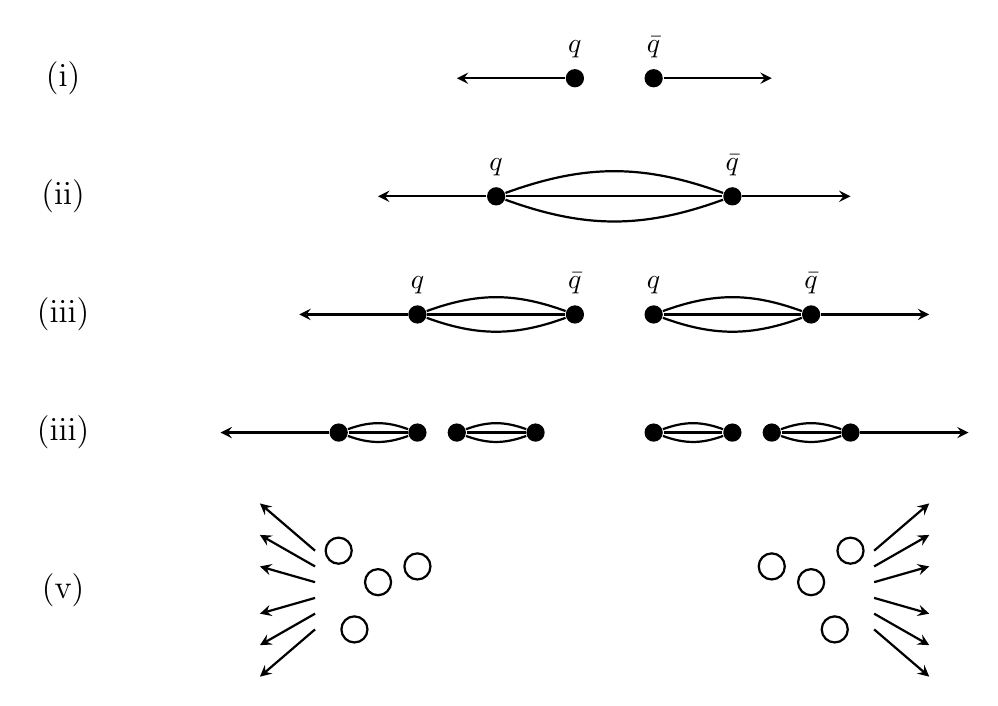
\begin{tikzpicture}[>=stealth,thick]

%----------------- (i) -----------------%
\node at (-2,0) {\large (i)};
% Quark & antiquark with arrows
\node[circle, fill=black, scale=0.7, label=above:$q$] (q_i) at (4.5,0) {};
\node[circle, fill=black, scale=0.7, label=above:$\bar{q}$] (qb_i) at (5.5,0) {};
\draw[->] (q_i) -- ++(-1.5, 0);
\draw[->] (qb_i) -- ++(+1.5, 0);

%----------------- (ii) -----------------%
\node at (-2,-1.5) {\large (ii)};
% Another q/qbar pair with a flux tube (string)
\node[circle, fill=black, scale=0.7, label=above:$q$] (q_ii) at (3.5,-1.5) {};
\node[circle, fill=black, scale=0.7, label=above:$\bar{q}$] (qb_ii) at (6.5,-1.5) {};
% Draw the string (solid line) plus double arrow to suggest tension
\draw[thick] (q_ii) to[out=20, in=160] (qb_ii);
\draw[thick] (q_ii) to[out=-20, in=-160] (qb_ii);
\draw (q_ii) -- (qb_ii);
\draw[->] (q_ii) -- ++(-1.5, 0);
\draw[->] (qb_ii) -- ++(+1.5, 0);

%----------------- (iii) -----------------%
\node at (-2,-3.0) {\large (iii)};
% Multiple q/qbar pairs horizontally
\node[circle, fill=black, scale=0.7, label=above:$q$] (q1_iii)  at (2.5, -3.0) {};
\node[circle, fill=black, scale=0.7, label=above:$\bar{q}$] (qb1_iii) at (4.5, -3.0) {};
\node[circle, fill=black, scale=0.7, label=above:$q$] (q2_iii)  at (5.5, -3.0) {};
\node[circle, fill=black, scale=0.7, label=above:$\bar{q}$] (qb2_iii)at (7.5, -3.0) {};

\draw[thick] (q1_iii) to[out=20, in=160] (qb1_iii);
\draw[thick] (q1_iii) to[out=-20, in=-160] (qb1_iii);
\draw[thick] (q2_iii) to[out=20, in=160] (qb2_iii);
\draw[thick] (q2_iii) to[out=-20, in=-160] (qb2_iii);

\draw (q1_iii) -- (qb1_iii);
\draw (q2_iii) -- (qb2_iii);

\draw[->] (q1_iii) -- ++(-1.5, 0);
\draw[->] (qb2_iii) -- ++(+1.5, 0);

%----------------- (iv) -----------------%
\node at (-2,-4.5) {\large (iii)};
% Multiple q/qbar pairs horizontally
\node[circle, fill=black, scale=0.7] (q11_iv)  at (1.5, -4.5) {};
\node[circle, fill=black, scale=0.7] (qb11_iv) at (2.5, -4.5) {};
\node[circle, fill=black, scale=0.7] (q12_iv)  at (3, -4.5) {};
\node[circle, fill=black, scale=0.7] (qb12_iv) at (4, -4.5) {};

\node[circle, fill=black, scale=0.7] (q21_iv)  at (5.5, -4.5) {};
\node[circle, fill=black, scale=0.7] (qb21_iv)at (6.5, -4.5) {};
\node[circle, fill=black, scale=0.7] (q22_iv)  at (7, -4.5) {};
\node[circle, fill=black, scale=0.7] (qb22_iv)at (8, -4.5) {};

\draw[thick] (q11_iv) to[out=20, in=160] (qb11_iv);
\draw[thick] (q11_iv) to[out=-20, in=-160] (qb11_iv);
\draw[thick] (q12_iv) to[out=20, in=160] (qb12_iv);
\draw[thick] (q12_iv) to[out=-20, in=-160] (qb12_iv);

\draw[thick] (q21_iv) to[out=20, in=160] (qb21_iv);
\draw[thick] (q21_iv) to[out=-20, in=-160] (qb21_iv);
\draw[thick] (q22_iv) to[out=20, in=160] (qb22_iv);
\draw[thick] (q22_iv) to[out=-20, in=-160] (qb22_iv);

\draw (q11_iv) -- (qb11_iv);
\draw (q12_iv) -- (qb12_iv);
\draw (q21_iv) -- (qb21_iv);
\draw (q22_iv) -- (qb22_iv);

\draw[->] (q11_iv) -- ++(-1.5, 0);
\draw[->] (qb22_iv) -- ++(+1.5, 0);
%----------------- (v) -----------------%
\node at (-2,-6.5) {\large (v)};
% Final hadrons on the left
\node[draw, circle, scale=1.0] (H1_v) at (1.5,-6) {};
\node[draw, circle, scale=1.0] (H2_v) at (1.7,-7) {};
\node[draw, circle, scale=1.0] (H3_v) at (2.5,-6.2) {};
\node[draw, circle, scale=1.0] (H4_v) at (2,-6.4) {};

% Arrows indicating motion outward
\draw[->] (1.2,-6) -- ++(-0.7, 0.6);
\draw[->] (1.2,-6.2) -- ++(-0.7, 0.4);
\draw[->] (1.2,-6.4) -- ++(-0.7, 0.2);
\draw[->] (1.2,-6.6) -- ++(-0.7, -0.2);
\draw[->] (1.2,-6.8) -- ++(-0.7, -0.4);
\draw[->] (1.2,-7) -- ++(-0.7, -0.6);

% Final hadrons on the right
\node[draw, circle, scale=1.0] (H5_v) at (8,-6) {};
\node[draw, circle, scale=1.0] (H6_v) at (7.8,-7) {};
\node[draw, circle, scale=1.0] (H7_v) at (7,-6.2) {};
\node[draw, circle, scale=1.0] (H8_v) at (7.5,-6.4) {};
\draw[->] (8.3,-6) -- ++(0.7, 0.6);
\draw[->] (8.3,-6.2) -- ++(0.7, 0.4);
\draw[->] (8.3,-6.4) -- ++(0.7, 0.2);
\draw[->] (8.3,-6.6) -- ++(0.7, -0.2);
\draw[->] (8.3,-6.8) -- ++(0.7, -0.4);
\draw[->] (8.3,-7) -- ++(0.7, -0.6);

\end{tikzpicture}